% \appendix

\chapter{Appendix: Modulation and Spectrum Simulation}

\section{Interactive OFDM Simulation Notebook}

To solidify the understanding of OFDM signal structure and spectral characteristics, an interactive Python notebook titled \texttt{A2-ofdm\_simulation.ipynb} is provided. This notebook allows learners to:

\begin{itemize}
  \item Visualize subcarriers of OFDM symbols.
  \item Explore Inverse Fast Fourier Transform (IFFT) as a modulation mechanism.
  \item Understand the effect of symbol length and guard intervals.
  \item Plot time and frequency domain representations.
\end{itemize}

\textbf{Notebook Access:}  
You can download the notebook from the following location:  
\url{<YOUR-LINK-TO-NOTEBOOK>}

\subsection{Modulation Scheme Explorer (Optional Streamlit App)}

For learners who prefer hands-on exploration, an interactive web application \texttt{ModulationExplorer.py} is also available. It allows users to experiment with:

\begin{itemize}
  \item QPSK, 16-QAM, and 64-QAM constellations.
  \item Variable number of symbols and noise levels.
  \item Visualization of signal degradation due to noise.
\end{itemize}

\begin{figure}[h!]
  \centering
  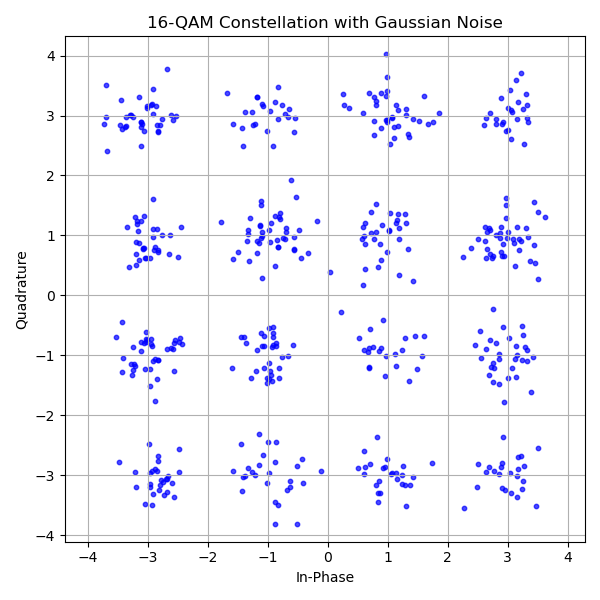
\includegraphics[width=0.8\textwidth]{figures/modulation_constellation_example.png}
  \caption{Example QAM constellation with added Gaussian noise (from Streamlit app).}
  \label{fig:modulation-app}
\end{figure}

\textbf{App Access:}  
Run the Streamlit app using the following command:
\begin{verbatim}
streamlit run ModulationExplorer.py
\end{verbatim}

\textbf{App Download:}  
\url{<YOUR-LINK-TO-APP-CODE>}

\subsection{Learning Outcomes}

\begin{itemize}
  \item Experience the spectral efficiency of OFDM in practice.
  \item Understand modulation scheme differences in terms of constellation design and noise resilience.
  \item Gain intuition about bit-symbol mappings and symbol space in the IQ-plane.
\end{itemize}

\textbf{Recommended Exercises:}
\begin{enumerate}
  \item Modify the number of subcarriers in the OFDM notebook and observe spectral changes.
  \item Change modulation order in the Streamlit app and analyze BER qualitatively.
\end{enumerate}
